\chapter[Lezione XI]{Lezione XI\newline\small{\emph{06/03/2011}}}
	\section{Lezione pre-esame}
Per un manuale affidabile sulla sintassi in C, è possibile fare riferimento alla voce \lstinline!C syntax! su \href{http://en.wikipedia.org/wiki/Main_Page}{Wikipedia} (in inglese).
		\subsection{Modello (o struttura) dei dati}
Le strutture dati studiate finora sono le seguenti (tranne le ultime due, cui s'accennerà in seguito):
\begin{itemize}[noitemsep]
	\item
Array o vettori, matrici (vedi il paragrafo~\vref{subsec:array});
	\item
Grafi (vedi il paragrafo~\vref{subsec:grafo});
	\item
Record o strutture (vedi il paragrafo~\vref{subsec:record});
	\item
Stack (vedi il paragrafo~\vref{subsec:stack});
	\item
Liste concatenate (vedi il paragrafo~\vref{subsec:liste});
	\item
Code (vedi il paragrafo~\vref{subsec:coda});
	\item
Alberi (vedi il paragrafo~\vref{subsec:albero}).
\end{itemize}
Ciascuno di questi modelli si caratterizza per le operazioni che permette di compiere. Nelle liste concatenate trattate nel  paragrafo~\vref{subsec:stack}, ad esempio, sono definiti l'inserimento (con la funzione \lstinline!push()!) e la cancellazione di elementi (tramite la funzione \lstinline!pop()!).

In ogni caso, una struttura dati non è troppo vincolante: è possibile creare una lista concatenata usando una matrice, ad esempio. Dichiarando una matrice di $n$ righe, si possono destinare le prime $n-1$ al ""carico utile'' e l'$n$-esima a puntare al nodo successivo. In parole povere, si usa l'$n$-esima riga come campo \lstinline!*next!. Così facendo, è come se una colonna di una matrice rappresentasse un nodo. Tuttavia, poiché le matrici sono indicizzate tramite interi $z$ progressivi, basterà un intero per identificare l'indirizzo del nodo successivo. Come ultimo accorgimento, basta stabilire che il nodo ""di coda'' contenga nella sua $n$-esima riga un intero negativo (come \lstinline!-1!) ad indicare la fine della lista. Ad ogni modo, servirà comunque una variabile ausiliaria (analogamente al puntatore \lstinline!*testa!) di tipo \lstinline!int! che indichi qual è il primo nodo.

Per l'esame, potrebbe essere necessario apportare delle modifiche ad una struttura dati esistente, come creare una lista concatenata bidirezionale (vedi la figura~\vref{fig:blist}). Tale struttura ha bisogno di due campi puntatore (\lstinline!*prev! e \lstinline!*next!) e può essere percorsa in entrambi i versi. Oppure, si potrebbero dover dichiarare più campi puntatori all'interno di un record per ordinare la lista in base a criteri differenti.

	\section{Strutture dati}
		\subsection{Coda}
		\label{subsec:coda}
La \emph{coda} (figura~\vref{fig:coda}) è una struttura dinamica lineare: gli elementi, cioè, sono ordinati. A differenza di uno stack, tuttavia, essi seguono una disciplina del tipo FIFO (\emph{First In First Out}). Un nuovo oggetto inserito si colloca in fondo alla coda, mentre per estrarne uno lo si preleva dalla testa.

Risulta ora evidente l'analogia di tale struttura con una fila (o coda) reale che si fa per usufruire di un servizio ad uno sportello, da cui peraltro prende il nome. Differenze tra coda e stack si riscontrano anche nel \emph{costo computazionale}, ossia sul numero di ""calcoli'' che l'esecutore deve compiere per effettuare un'operazione sulla struttura, come mostra la tabella ~\vref{tab:co-st}. Per eliminare un elemento, partendo da \lstinline!*testa!, il computer deve percorrere tutta la coda finché non giunge all'ultimo. Per ""snellire'' il costo computazionale della coda, è possibile introdurre un puntatore al nodo finale in modo tale che l'eliminazione comporti un solo passaggio, al pari dell'inserimento.

		\subsection{Albero}
		\label{subsec:albero}
Un \emph{albero} è un modello dei dati che sfrutta una struttura gerarchica. Esistono diverse implementazioni di albero; in prima battuta si può considerare una rappresentazione che preveda due campi puntatore per ogni struttura. Siano essi \lstinline!*min! e \lstinline!*max!.

Si supponga di aver bisogno di tenere ordinati $n$ dati numerici inseriti nello \lstinline!stdin!. All'inserimento del primo dato $d_1$ si crea un nodo (sia esso \lstinline!n_1!), chiamato \emph{capostipite} o \emph{padre} (il ""pallino'' rosso in figura~\vref{fig:albero}). All'ingresso del secondo dato $d_2$ si crea un altro nodo (\lstinline!n_2!) e si stabilisce che:
\begin{itemize}
	\item
$d_1>d_2 \quad \rightarrow \quad $ \lstinline!min = &n_2!;
	\item
$d_1<d_2 \quad \rightarrow \quad $ \lstinline!max = &n_2!.
\end{itemize}
Ripetendo il procedimento $n$ volte, si avranno dei record contenenti numeri ordinati (in ordine crescente, in questo caso).

%\begin{wrapfloat}{figure}{o}{0pt}
%	\centering
%	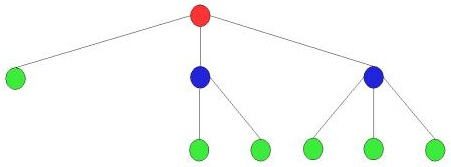
\includegraphics[width=0.5\columnwidth]{immagini/albero}
%	\caption[Albero]{Rappresentazione grafica di un albero}
%	%\label{fig:albero}
%\end{wrapfloat}

Per com'è stato costruito quest'albero, ogni {\em genitore} può essere collegato al massimo a due \emph{figli}. Esso è, quindi, un albero binario o BST (\emph{Binary Search Tree}, figura~\vref{fig:bst1}). Ad ogni modo, è possibile creare una struttura ""dal basso'', in cui ogni albero figlio ha un puntatore al genitore. Tale modifica permette di avere un albero non più (soltanto) binario ma anche a più elementi.

\begin{table}
	\centering
	\caption[Costo computazionale]{La tabella mostra il costo computazionale di uno stack, una coda ed una coda con un puntatore all'ultimo elemento, con $n$ elementi.}
	\label{tab:co-st}
	\begin{tabular}{l | c c}
		\toprule
\emph{Struttura}		&\emph{Inserimento}	&\emph{Eliminazione}	\\
		\midrule
	Stack			&$1$				&$1$				\\
	Coda			&$n$				&$1$				\\
	Coda (puntatore)	&$1$				&$1$
	\end{tabular}
\end{table}

\begin{figure}
	\centering
\subfloat[Binary Search Tree][\emph{Binary Search Tree}\label{fig:bst1}]{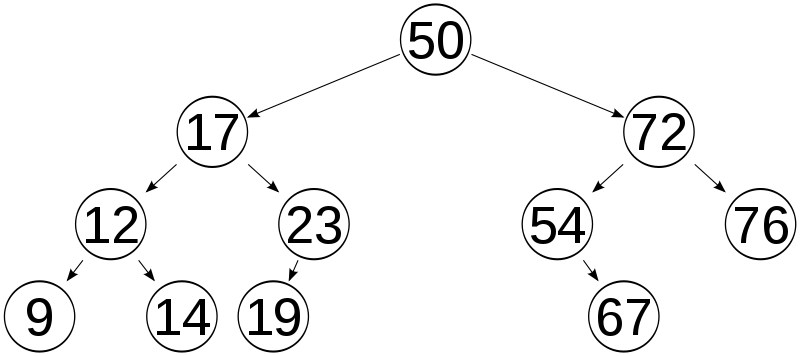
\includegraphics[width=\columnwidth]{immagini/bst_1}} \\
\subfloat[BST con caratteri alfabetici][\emph{BST con caratteri alfabetici}\label{fig:bst_2}]{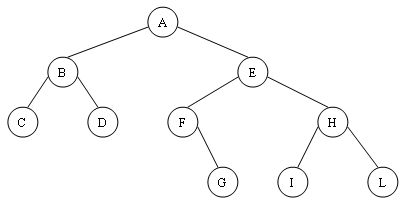
\includegraphics[width=0.45\columnwidth]{immagini/bst_2}} \quad
\subfloat[Albero][\emph{Rappresentazione grafica di un albero}\label{fig:albero}]{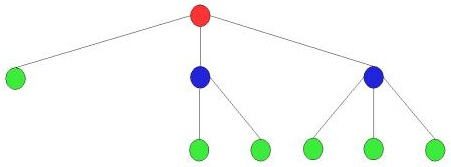
\includegraphics[width=0.45\columnwidth]{immagini/albero}}\\
\subfloat[Lista concatenata bidirezionale][{\em Lista concatenata bidirezionale. I campi in blu sono puntatori.}\label{fig:blist}]{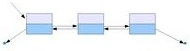
\includegraphics[width=0.45\columnwidth]{immagini/lista_bidirezionale}}\quad
\subfloat[Coda][{\em Rappresentazione grafica di una coda.}\label{fig:coda}]{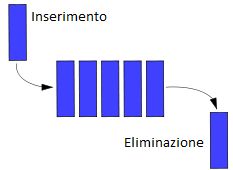
\includegraphics[width=0.45\columnwidth]{immagini/coda}}
	\caption{Alcune strutture dati.}
\end{figure}